\documentclass{sig-alternate}
\usepackage{url}
\usepackage{pgffor}
\usepackage[font=bf]{caption}
\usepackage{subcaption}
\usepackage[usenames,dvipsnames,svgnames,table]{xcolor}
\usepackage{bm}
\usepackage{balance}
\usepackage{xcolor}

\setcopyright{acmcopyright}
\conferenceinfo{GECCO '15,}{July 11 - 15, 2015, Madrid, Spain}
\isbn{978-1-4503-3472-3/15/07}\acmPrice{\$15.00}
\doi{http://dx.doi.org/10.1145/2739480.2754731}

\clubpenalty=10000 
\widowpenalty = 10000

\begin{document}

\title{Novelty Search for Soft Robotic Space Exploration}
%\subtitle{[Extended Abstract]
%\titlenote{A full version of this paper is available as
%\textit{Author's Guide to Preparing ACM SIG Proceedings Using
%\LaTeX$2_\epsilon$\ and BibTeX} at
%\texttt{www.acm.org/eaddress.htm}}}
\numberofauthors{4}
\author{
% You can go ahead and credit any number of authors here,
% e.g. one 'row of three' or two rows (consisting of one row of three
% and a second row of one, two or three).
%
% The command \alignauthor (no curly braces needed) should
% precede each author name, affiliation/snail-mail address and
% e-mail address. Additionally, tag each line of
% affiliation/address with \affaddr, and tag the
% e-mail address with \email.
\alignauthor
Georgios Methenitis\titlenote{Based on the master's thesis~\cite{methenitis2014evolution}, work conducted under the supervision of both the University of Amsterdam and the Advanced Concepts Team (ESTEC).}\\
       \affaddr{Centrum Wiskunde \& Informatica}\\
       \affaddr{(CWI)}\\
       \affaddr{Amsterdam, The Netherlands}\\[0.05cm]
       \email{\hspace{-0.5cm}Georgios.Methenitis@cwi.nl~}
 % 2nd. author
\alignauthor
Daniel Hennes\\
       \affaddr{Advanced Concepts Team}\\
       \affaddr{European Space Agency (ESTEC)}\\
       \affaddr{Noordwijk, The Netherlands}\\
       \email{Daniel.Hennes@esa.int}
  % 3rd. author
\alignauthor
Dario Izzo\\
       \affaddr{Advanced Concepts Team}\\
       \affaddr{European Space Agency (ESTEC)}\\
       \affaddr{Noordwijk, The Netherlands}\\
       \email{Dario.Izzo@esa.int}
\and  % use '\and' if you need 'another row' of author names
% 4th. author
\alignauthor 
Arnoud Visser\\
       \affaddr{University of Amsterdam}\\
       \affaddr{Amsterdam, The Netherlands}\\[0.05cm]
       \email{A.Visser@uva.nl}
}


\begin{CCSXML}
<ccs2012>
<concept>
<concept_id>10010147.10010178</concept_id>
<concept_desc>Computing methodologies~Artificial intelligence</concept_desc>
<concept_significance>500</concept_significance>
</concept>
<concept>
<concept_id>10010147.10010178.10010199.10010204.10011814</concept_id>
<concept_desc>Computing methodologies~Evolutionary robotics</concept_desc>
<concept_significance>500</concept_significance>
</concept>
<concept>
<concept_id>10010147.10010178.10010205</concept_id>
<concept_desc>Computing methodologies~Search methodologies</concept_desc>
<concept_significance>500</concept_significance>
</concept>
<concept>
<concept_id>10010147.10010178.10010213</concept_id>
<concept_desc>Computing methodologies~Control methods</concept_desc>
<concept_significance>500</concept_significance>
</concept>
</ccs2012>
\end{CCSXML}

\ccsdesc[500]{Computing methodologies~Artificial intelligence}
\ccsdesc[500]{Computing methodologies~Evolutionary robotics}
\ccsdesc[500]{Computing methodologies~Search methodologies}
\ccsdesc[500]{Computing methodologies~Control methods}

\maketitle
\begin{abstract}
The use of soft robots in future space exploration is still a far-fetched idea, but an attractive one. Soft robots are inherently compliant mechanisms that are well suited for locomotion on rough terrain as often faced in extra-planetary environments. Depending on the particular application and requirements, the best shape (or body morphology) and locomotion strategy for such robots will vary substantially. Recent developments in soft robotics and evolutionary optimization showed the possibility to simultaneously evolve the morphology and locomotion strategy in simulated trials. The use of techniques such as generative encoding and neural evolution were key to these findings. In this paper, we improve further on this methodology by introducing the use of a novelty measure during the evolution process. We compare fitness search and novelty search in different gravity levels and we consistently find novelty--based search to perform as good as or better than a fitness--based search, while also delivering a greater variety of designs. We propose a combination of the two techniques using fitness--elitism in novelty search to obtain a further improvement. We then use our methodology to evolve the gait and morphology of soft robots at different gravity levels, finding a taxonomy of possible locomotion strategies that are analyzed in the context of space-exploration.
\end{abstract}

\printccsdesc

\keywords{soft robotics, locomotion, novelty search, CPPN, CPPN-NEAT, VoxCAD, space exploration}

\section{Introduction}
Robotic exploration of extraterrestrial bodies is a challenging endeavour that requires the deployment of advanced technological solutions. The Huygens descent on Titan, the landing of Philae on the comet 67P/Churyumov-Gerasimenko or the daily accounts of the three martian rovers Spirit, Opportunity and Curiosity are incredible achievements that were made possible by our ever increasing technological capabilities. One challenge, in all of these missions, is that of mobility. Advanced mobility solutions for exoplanetary rovers are the subject of active research. It is not uncommon in this research field to find ideas drawing inspiration from biology. For example, this was the case for the Mars tumbleweed exploration concept \cite{antol2003low, ylikorpi2004biologically}, the lunar ALI exploration concept \cite{clark2005ali}, or the many legged robots, inspired by insect locomotion, that are being studied in the context of exoplanetary exploration. The locomotion strategy and the body morphology of these robots, though closely related, were not co-designed and were treated as rather uncoupled entities. In this work, we are interested in investigating the possibility to simultaneously design the morphology and the gait of robots as to adapt their locomotion to different extraterrestrial environments defined by different terrain types and gravity strengths. The effects of gravity, slopes, and stiffness on the gaits evolved by a quadruped robot in dynamic walking and running was researched in~\cite{papadopoulos2013ariadna, kontolatisquadruped}. Hildebrand gait diagrams~\cite{Hildebrand1989-HILVLA} were employed to analyze gaits and prove their stability under varying planetary conditions. The robot morphology, though, was kept fixed and only the leg lengths and the controller were subject to optimization. The simultaneous optimization of gaits and morphology, using evolutionary techniques is, though, possible. In the work of Sims~\cite{sims1994evolving} a generative (or indirect) encoding was used to enable the evolution of virtual creatures adapted for jumping, walking or swimming. The idea has been a source of inspiration for a large number of later works and recently, the practical possibility to evolve soft material robots~\cite{hiller2012automatic} able to produce locomotion has been proved. The evolution of soft structures in a virtual environment was later also studied in~\cite{cheney2013unshackling} where a powerful generative encoding, CPPNs~\cite{stanley2007compositional}, was used to generate soft voxel-formed three dimensional structures, coupled with the use of NEAT algorithm which ensures the increasing complexity of the networks produced.  
The interest of soft robotics~\cite{trivedi2008soft, pfeifer2012challenges} for space exploration has been recently well defined by Lin, Leisk and Trimmer \cite{softrobotsinspace} and summarized in three points: a) intrinsically safe (rather than \lq\lq control safe\rq\rq) b) morph-able (size-changing and versatile) and c) gravity independent (able to move in any orientation).  Having no rigid parts in their design (See Fig.~\ref{fig:softRobotsActuation}), the degrees of freedom of a soft robot are infinite and the possible ways of motion can become extremely rich and hard to control. 
In this paper we build upon previous work~\cite{cheney2013unshackling} first improving significantly the methodology by considering the evolutionary process as driven by novelty~\cite{lehman2008exploiting,lehman2011abandoning,lehman2010revising, risi2009novelty} rather than by fitness. A similar idea was investigated in~\cite{lehman2011evolving} in the context of rigid robots and proved to result in a far more exploratory algorithm in the space of morphologies. We then obtain a further performance boost combining novelty search with fitness--elitism and we use the resulting algorithm to evolve a number of robots and locomotion patterns adapted to different planetary conditions. Given the extreme complexity of the task and the early research stages of the tools used, we are not as much interested in the practical use of the designs evolved as in their use to inspire future advanced robotic exploration missions.

\begin{figure}[t!]
\centering
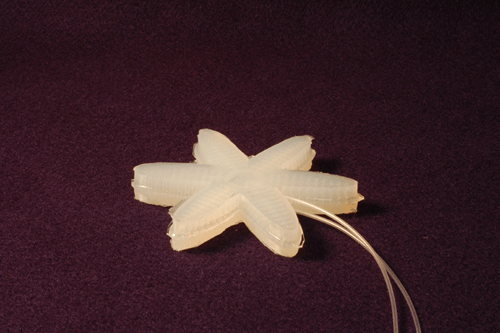
\includegraphics[width=0.22\textwidth,height=0.12\textheight]{../Figures/Misc/soft_robotics_figure.png}\		
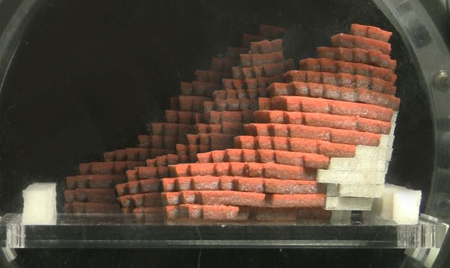
\includegraphics[width=0.22\textwidth,height=0.12\textheight]{../Figures/Misc/hillerPressureChamber.png}\\[0.1cm]	
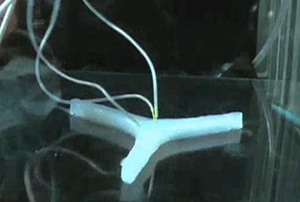
\includegraphics[width=0.22\textwidth,height=0.12\textheight]{../Figures/Misc/ExplodingRobot.jpg}\	
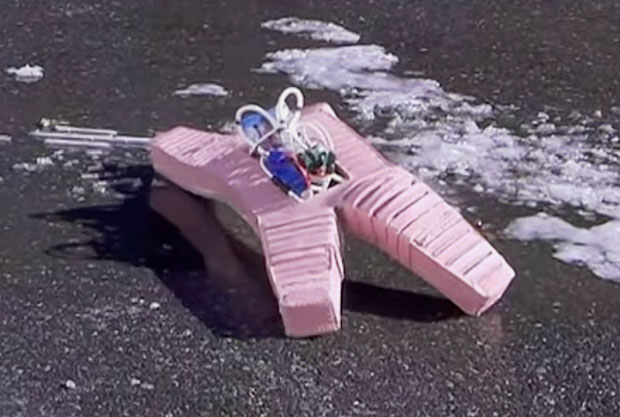
\includegraphics[width=0.22\textwidth,height=0.12\textheight]{../Figures/Misc/softbot.jpg}\\
\caption{Soft robots can be actuated through air pressure tubes (top-left), pressure variations (top-right), or internal explosions (bottom-left). Autonomously actuated soft robot~\cite{tolley2014resilient}, it is able to withstand extreme temperatures and variant terrain types (bottom-right).}
\label{fig:softRobotsActuation}
\end{figure}


\section{Background}
We start by introducing VoxCad, the open source simulator used throughout this study to analyze soft robot morphologies and locomotion strategies. Shape and structure of the studied robots are expressed using a generative encoding technique and evolved using a neuro-evolutionary algorithm called CPPN-NEAT. In particular, we follow the approach detailed in previous work~\cite{cheney2013unshackling} and briefly summarize the key aspects of the resulting setup here.

%We make use of the open source VoxCad simulator~\cite{hiller2012dynamic} to evaluate soft robots in different environments\footnote{VoxCad can be downloaded at \url{http://www.voxcad.com/}}. Our soft robots bodies are built from a generative encoding representation based on CPPN. NEAT is then used to evolve the CPPN and thus generate new soft robots designs from previous generations. With this respect, our set-up is the same as that used in~\cite{cheney2013unshackling}. We thus here briefly describe the basic tools at the core of our research.
\newpage
\subsection{VoxCad simulator}
%Most work to simulate interactions and deformations within and between soft material bodies are focused on the graphical part of the problem~\cite{faloutsos1997dynamic} sacrificing the accuracy of the simulation~\cite{teschner2004versatile}. Three dimensional meshes~\cite{muller2002stable} can represent these bodies including the dynamics of their materials. 
VoxCad~\cite{hiller2012dynamic} is a simulator targeted to mimic the physics of soft material, while accurately reflecting deformations and interactions. The workspace is represented as a 3D-lattice, where each voxel is of a certain material type. Materials can be actuated (i.e. expansion or contraction) by an external trigger. External actuation is achieved by varying the temperature of the environment and thus exploiting the various material properties. Modifying the material properties results in soft or hard material that either does (active) or does not  react (passive) to temperature variations.
%\subsubsection*{Materials}
%Materials can be \emph{passive} or \emph{active} in respect to their reaction to the temperature changes. Passive materials do not react to temperature changes, while active materials expand and contract in respect to their thermal properties. \textcolor{Red}{Red} and \textcolor{Green}{Green} are the only actuated materials with non-zero and opposite thermal expansion coefficients. The two additional materials represent non-actuated tissue that can be soft (soft tissue) or hard (bones). \textcolor{Cyan}{Cyan} voxels are soft having five times smaller elastic modulus of their material than \textcolor{Blue}{Blue} which have $50$ \texttt{MPa}.

\begin{figure}[t!]
\centering
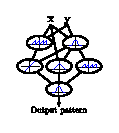
\includegraphics[width=0.15\textwidth]{../Figures/Misc/cppnNetwork.eps}
\caption{Compositional pattern-producing networks have identical network structure with artificial neural networks while they make use of a canonical set of activation functions.}
\label{fig:cppnNetwork}
\end{figure}


\begin{figure}[t!]
\vspace{1cm}
\centering
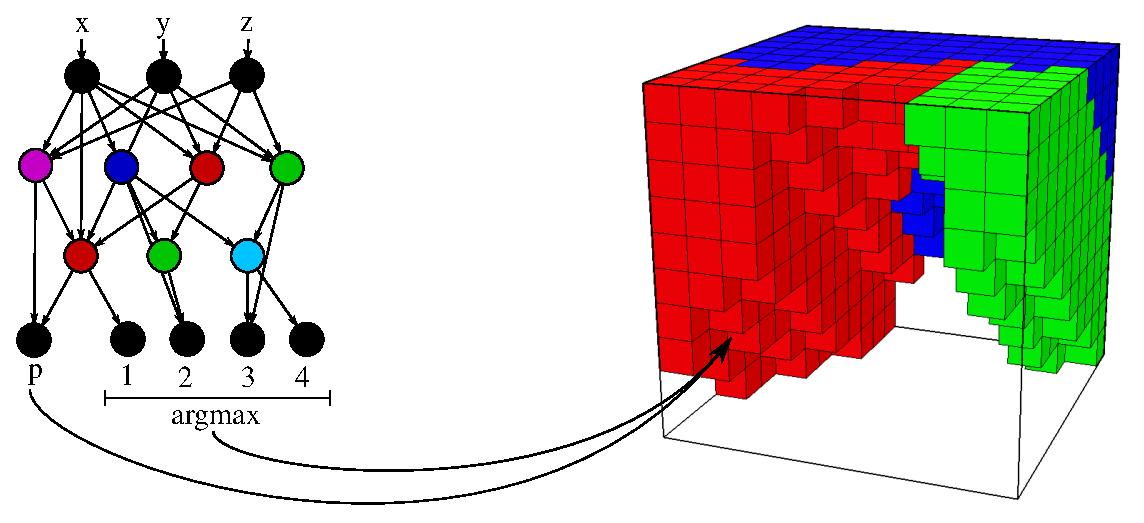
\includegraphics[width=0.35\textheight]{../Figures/Misc/cppnSoftBot.eps}
\caption{Each genotype (CPPN) is queried for every coordinate inside the lattice, its outputs determine the presence of a voxel and the type of its material.}
\label{fig:cppnDiagram}
\end{figure}

\subsection{Generative encoding}
We use the technique of Compositional Pattern-Producing Networks (CPPNs)~\cite{stanley2007compositional} as a generative encoding to produce morphologies (i.e. shape and structure) of simulated soft robots. CPPNs are artificial neural networks with an extended set of activation functions. The set of activation functions can include repetitive, symmetrical, and linear functions; an example is depicted in Figure~\ref{fig:cppnNetwork}. The CPPNs are queried for every coordinate of the lattice space to form a soft robot shape as well as to define the distribution of the materials. The input nodes (neurons) of the CPPN are assigned to normalized coordinates:\footnote{Therefore, the morphology can be sampled at different lattice resolutions.} $x,y,z \in [-1, 1]$. The output of the network defines if the queried voxel is enabled and which material is used. The generative encoding of voxelyzed soft robots through CPPNs is shown in Figure~\ref{fig:cppnDiagram}. 

%A bias input node is also introduced in the genome CPPN representation, this will allow the network to produce arbitrary outputs different from the defaults when all other inputs values are set to zero. 
%More inputs can be added to the CPPNs, for instance the distance from the center point of the Cartesian phenotype space (lattice) as described in~\cite{stanley2007compositional} and used in~\cite{cheney2013unshackling} which adds more bias towards symmetrical structures.
%The proposed input nodes for the three dimensions of the Cartesian space provide the minimum bias to the network outputs. Figure~\ref{fig:cppnDiagram} illustrates the topology of a random CPPN network with the input and output nodes  described earlier. The presence of a voxel in each coordinate of the lattice is determined by a single output of the CPPN, denoted with $p$ while the selection of the material is determined by $n$-outputs.
\newpage
\subsection{CPPN-NEAT}
As CPPNs are artificial neural networks, yet with a richer set of activation function, we can deploy neuro-evolutionary algorithms to evolve these networks. Specifically, we use a technique called NeuroEvolution of Augmenting Topologies (NEAT)~\cite{stanley2002evolving} with minor modifications in order to be applicable to CPPNs, the resulting algorithm is known as CPPN-NEAT~\cite{stanley2007compositional}. During evolution, CPPN-NEAT modifies not only the weights, but also the structure of the network and the activation functions. As such, the number of hidden layers and neurons does not need to be fixed in advance.
%Previous work~\cite{cheney2013unshackling}, showed that this method can indeed evolve the morphologies of the soft robots in the VoxCad simulation environment. 
%\textit{HyperNEAT}\footnote{HyperNEAT \texttt{v4.0 C++}  by J. Gauci code (url: \url{https://github.com/MisterTea/HyperNEAT})} is used for the implementation of the CPPN-NEAT algorithm.

\section{Methodology}
As outlined in the previous section, the use of soft robot simulator (VoxCad) and generative encoding in combination with neuro-evolution through CPPN-NEAT paves the way for successfully evolving complex morphologies for soft robots. However, in previous work~\cite{cheney2013unshackling}, the diversity of evolved creatures was limited. Different locomotion profiles were predominantly the result of including secondary costs (e.g., cost for actuated voxels or voxel connections) in the fitness function. We now describe our approach based on \textit{novelty search} that ensures intrinsic diversity without the need for a ``hand-coded'' objective that is subjective to the designers domain knowledge and may not generalize to exoplanetary environments with a variety of gravity levels. In addition, we describe how fitness--elitism can be incorporated in novelty search to combine the best of both worlds.

\subsection{Novelty search}

Unlike traditional fitness--based search, novelty search~\cite{lehman2008exploiting,lehman2011abandoning,lehman2010revising, risi2009novelty} is an alternative way of optimization. Novelty search, evaluates new candidates with respect to their ``novelty'' when compared to all previously found solutions and not based on an objective function. The ``novelty'' measure is defined in the behavior space, which is a function of the phenotype. As an example, one can think of the behavior as the trajectory of a robot controlled by a neural network. A ``novel'' candidate will exhibit a trajectory that differs from all previously recorded trajectories (i.e. in the behavior space) and novelty is not determined by the difference in the weights of the neural network (i.e the genome search space).

%To define novelty, a metric measures the difference in the behavior space of the phenotype. Given the phenotype's behavior $x$ a novelty measurement could be a function of $x$, $f(x)$ which computes how different (novel) is the specific behavior in respect to a set of other behaviors $S$ in behavior space.  As defined in~\cite{lehman2008exploiting,lehman2011abandoning} \emph{sparseness} can give a good measurement of how sparse is the area of a newly observed behavior. Given the behavior we can compute the sparseness by:

For a behavior $x$, a novelty measure $f(x)$ determines how different the specific behavior is in respect to a set of other behaviors $\mathcal{S}$. We follow the definition in~\cite{lehman2008exploiting,lehman2011abandoning}, where the novelty measure is defined as \emph{sparseness} measuring the average distance from the $k$--closest behaviors:
\begin{equation}
\label{sparsenessEquation}
f(x) = \cfrac{1}{k} \sum_{i=1}^{k} dist(x, \mathcal{S}_i)\ , 
\end{equation}
where $S$ is a sorted set of the closest behaviors and $dist$ is a distance function between two behaviors.


% Sparsity measures the average distance from the $k$-closest behaviors.

%\todo{I dont know what this means:} 
%One significant point here is that the behavior space in some domains can be limitless. However, a valid behavioral metric can be found by excluding behaviors that are meaningless or do not comply with the natural limits of the problem. On the other hand, the search space in the genotype level can also be infinite especially in neuroevolution methods like NEAT where the structure of neural networks can grow during the evolution. A bounded space of understandable-valid behaviors is then the key idea of novelty search where increasingly complex behaviors present to the evolution as the complexity of the genotype grows along.

%\subsubsection*{Behaviours in Novelty Search}

In the context of soft robots, we define a behavior as the way the robot interacts with the environment during a VoxCad simulation run. Every aspect of the soft robot movement that can be observed, can also be used to describe the behavior. 
% TODO: good point below, but rather for discussion not here, we just made the point that the novelty meassure is the behavior not the morphology!!!
%Previous work~\cite{lehman2011evolving} in a try to evolve walking three-dimensional virtual creatures used the evolved morphology of the creatures to describe their behavior. Although, comparing the morphology of the evolved soft robots is similar to comparing the chromosome (CPPN) of each individual. Behaviors that describe the morphology of the evolved robots have failed~\cite{lehman2011evolving}, since search is then forcing new types of morphologies without caring about the actual target of the evolution, which was the efficient locomotion. Therefore, only the comparison of the observed behavior in the phenotype level can lead the evolution towards more complex behaviors. 
It is expected that behaviors that indirectly contain fitness--related information (i.e. displacement) will be more successful in terms of the original fitness function. Figure~\ref{fig:Behaviors} presents all behaviors used for novelty computation during our study, in addition to behaviors that relate to displacement, e.g., trajectories and pace, we also include others that do not have this obvious relation, e.g., number of voxels touching the ground, kinetic energy, and pressure. For all recorded behavior metrics a constant sampling rate ensures that all signals have the same length. Furthermore, the discrete Fourier transformation of one dimensional signals was used to define other behavior types. The dominant frequencies of the pace, voxels touching the ground, pressure, and kinetic energy is expected to be descriptive of the locomotion strategies the evolved soft robots exhibit.


\begin{figure}[t!]
\centering
\begin{subfigure}[b]{0.47\textwidth}
\centering
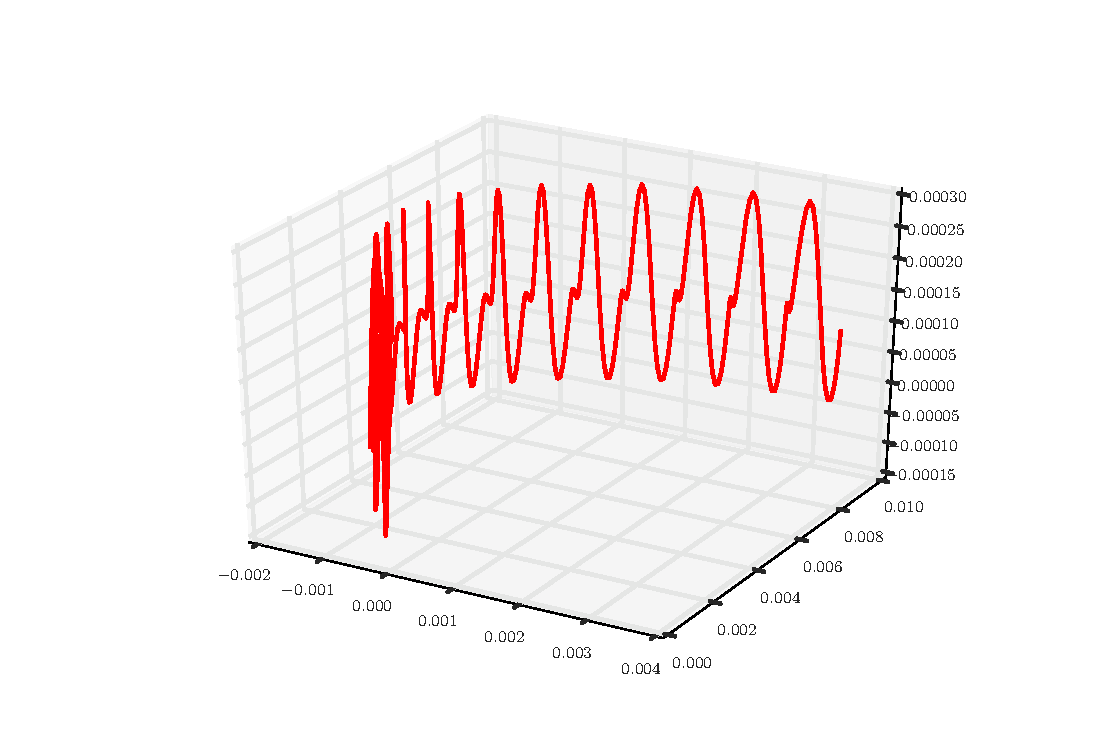
\includegraphics[width=0.49\textwidth]{../Figures/Behaviors/3d.pdf}
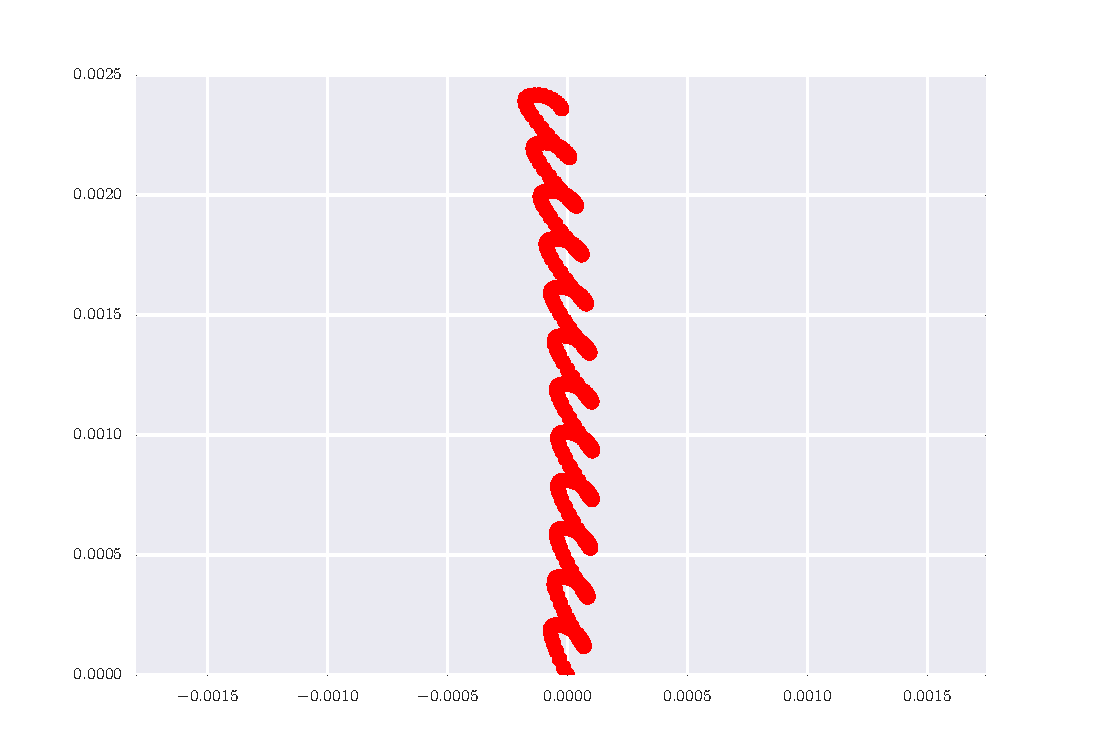
\includegraphics[width=0.49\textwidth]{../Figures/Behaviors/2d.pdf}
\caption{Three and two dimensional trajectories of the soft robots.}
\end{subfigure}
\begin{subfigure}[t]{0.23\textwidth}
\centering
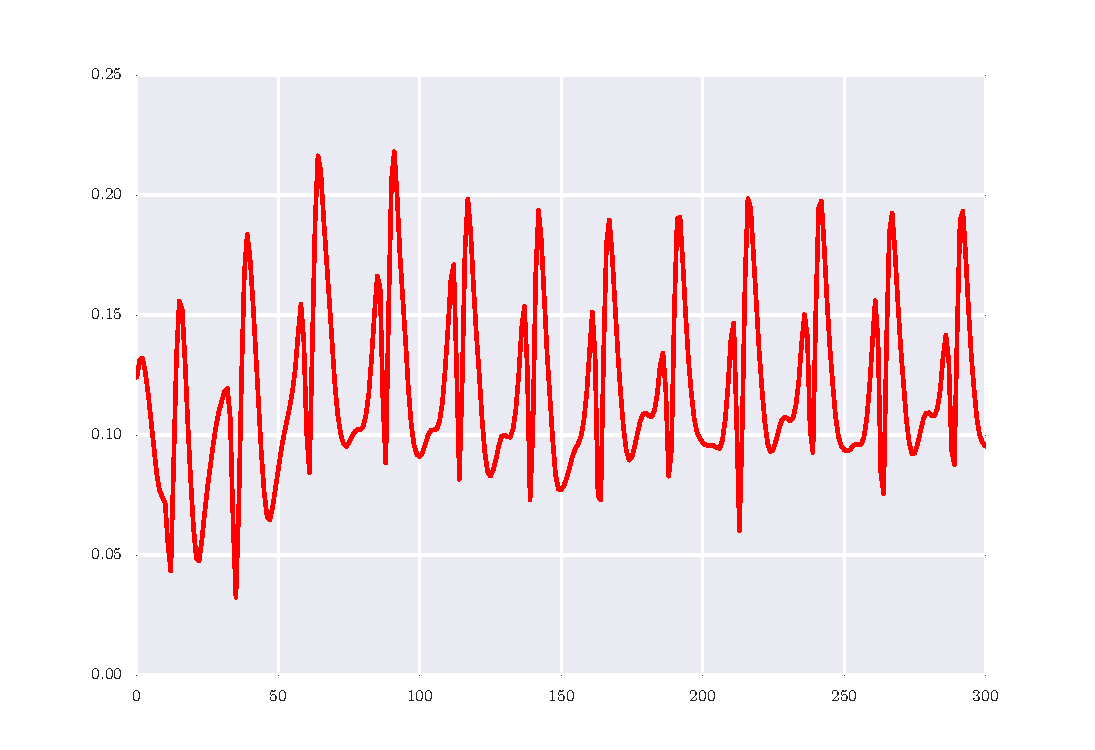
\includegraphics[width=0.5\textwidth]{../Figures/Behaviors/pace.pdf}~
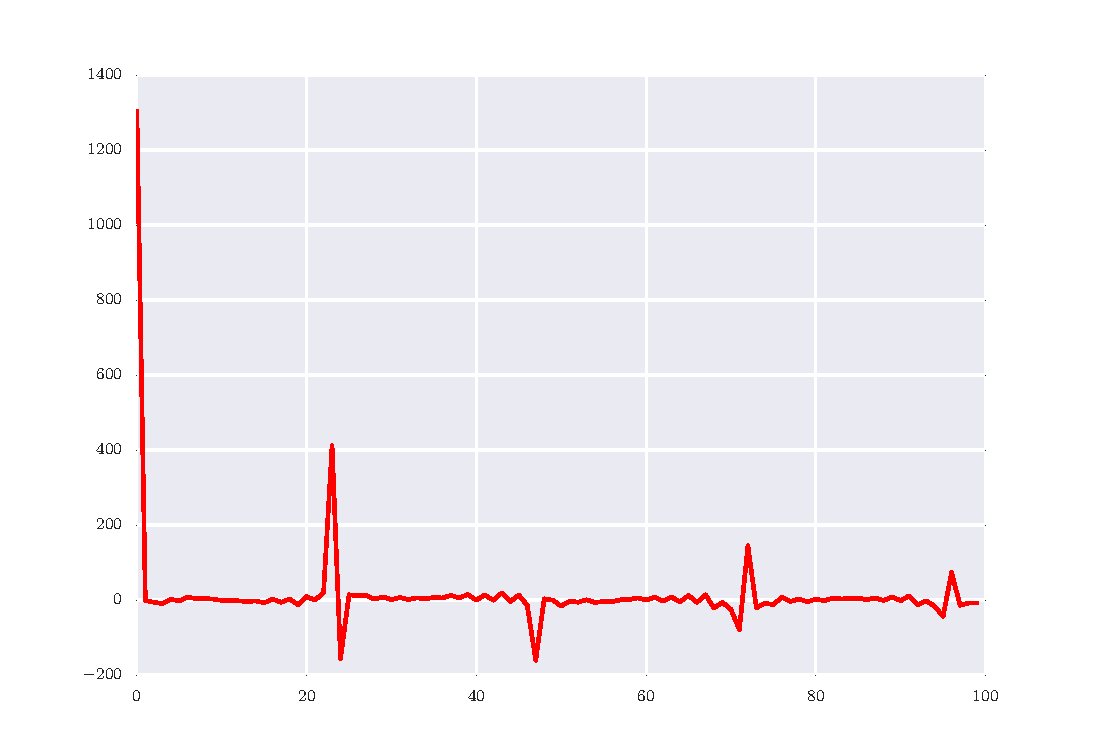
\includegraphics[width=0.5\textwidth]{../Figures/Behaviors/pacedft.pdf}
\caption{Pace and discrete Fourier transformation of the same signal.}
\end{subfigure}~
\begin{subfigure}[t]{0.23\textwidth}
\centering
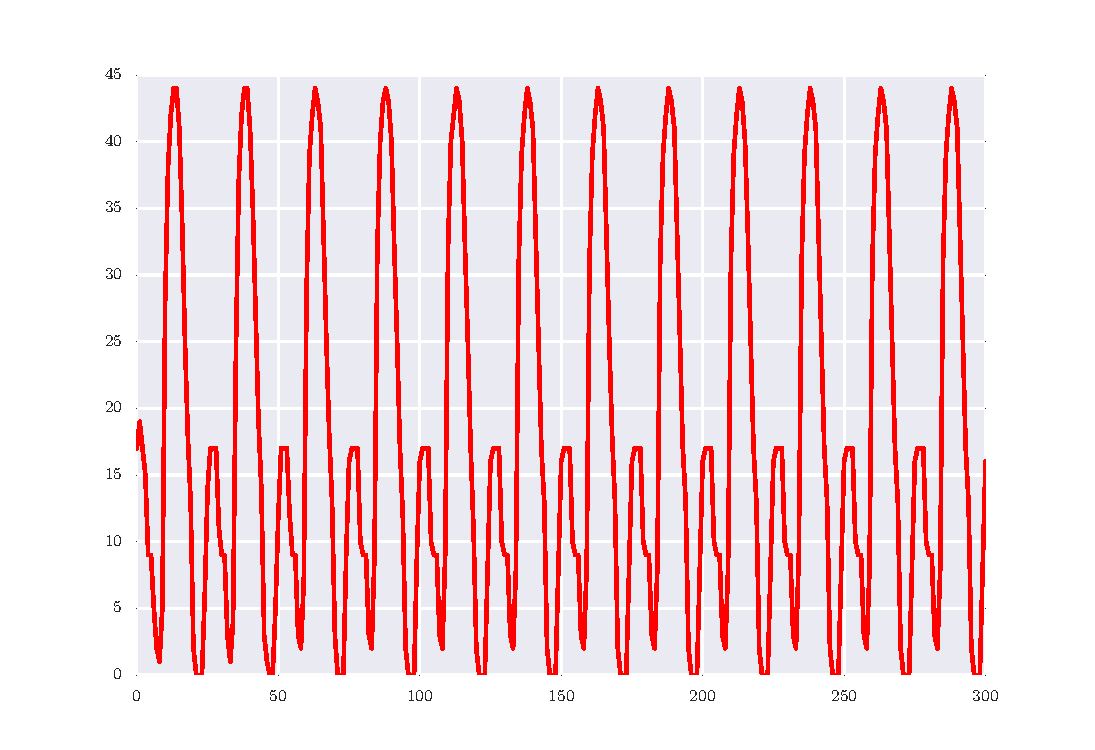
\includegraphics[width=0.5\textwidth]{../Figures/Behaviors/vtg.pdf}~
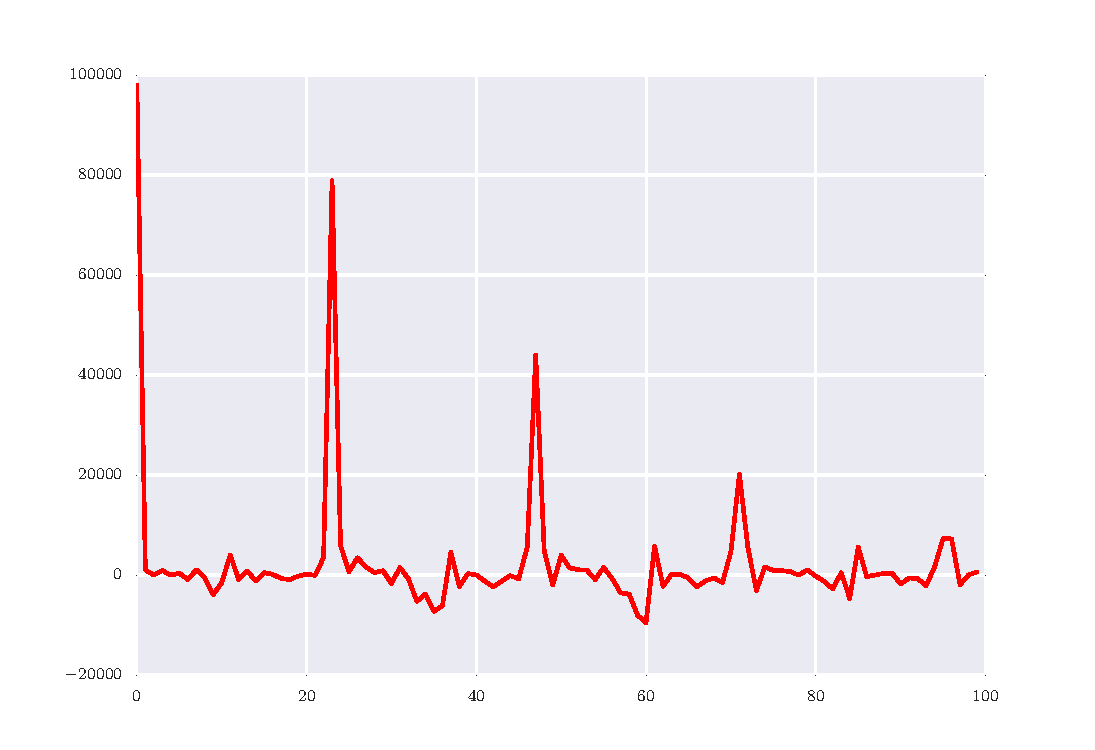
\includegraphics[width=0.5\textwidth]{../Figures/Behaviors/vtgdft.pdf}
\caption{Voxels touching the ground and discrete Fourier transformation of the same signal.}
\end{subfigure}\\
\begin{subfigure}[t]{0.23\textwidth}
\centering
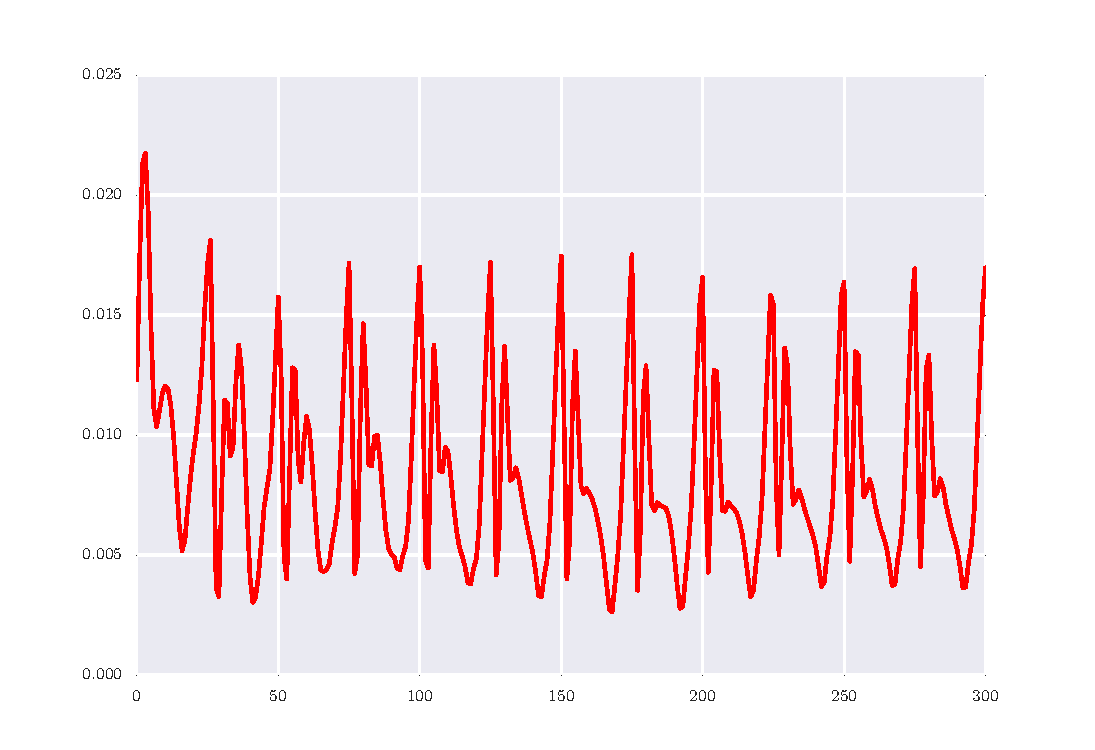
\includegraphics[width=0.5\textwidth]{../Figures/Behaviors/pr.pdf}~
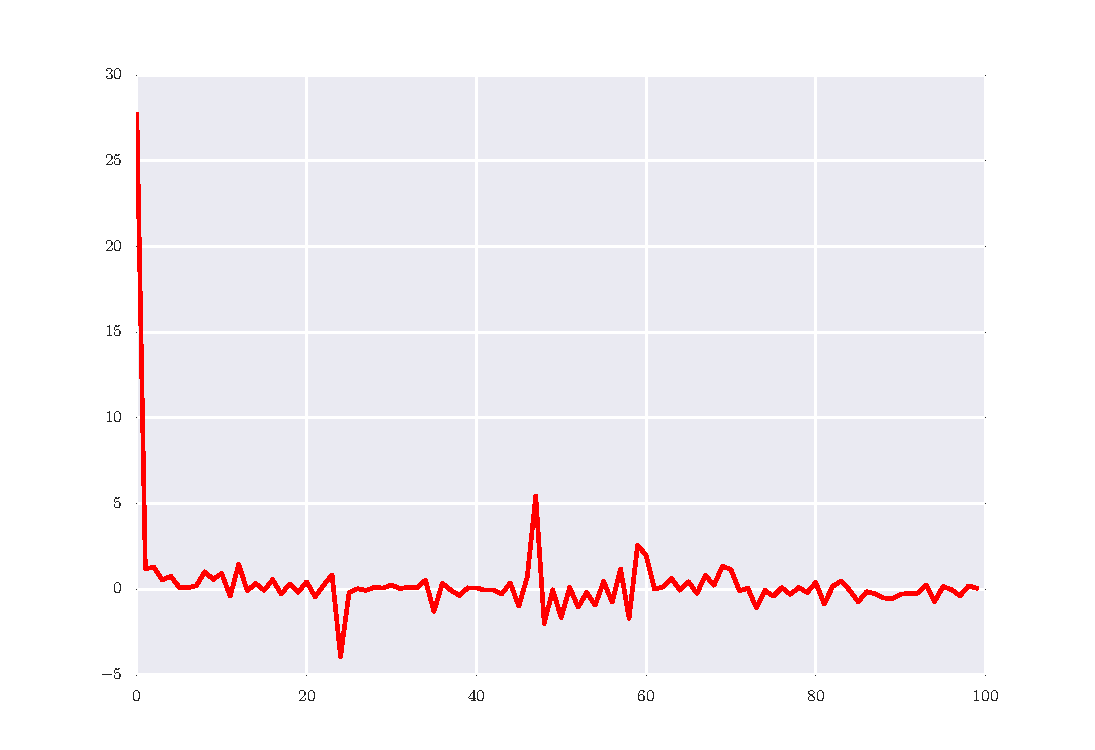
\includegraphics[width=0.5\textwidth]{../Figures/Behaviors/prdft.pdf}
\caption{Maximum pressure and discrete Fourier transformation of the same signal.}
\end{subfigure}~
\begin{subfigure}[t]{0.23\textwidth}
\centering
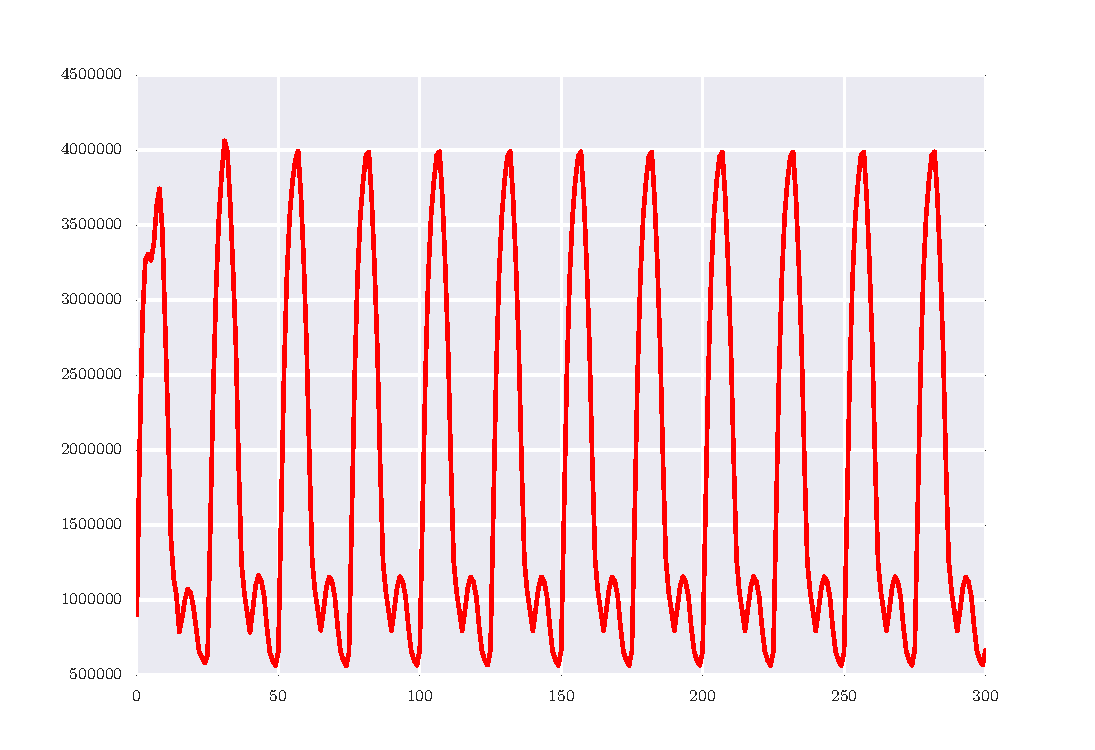
\includegraphics[width=0.5\textwidth]{../Figures/Behaviors/ke.pdf}~
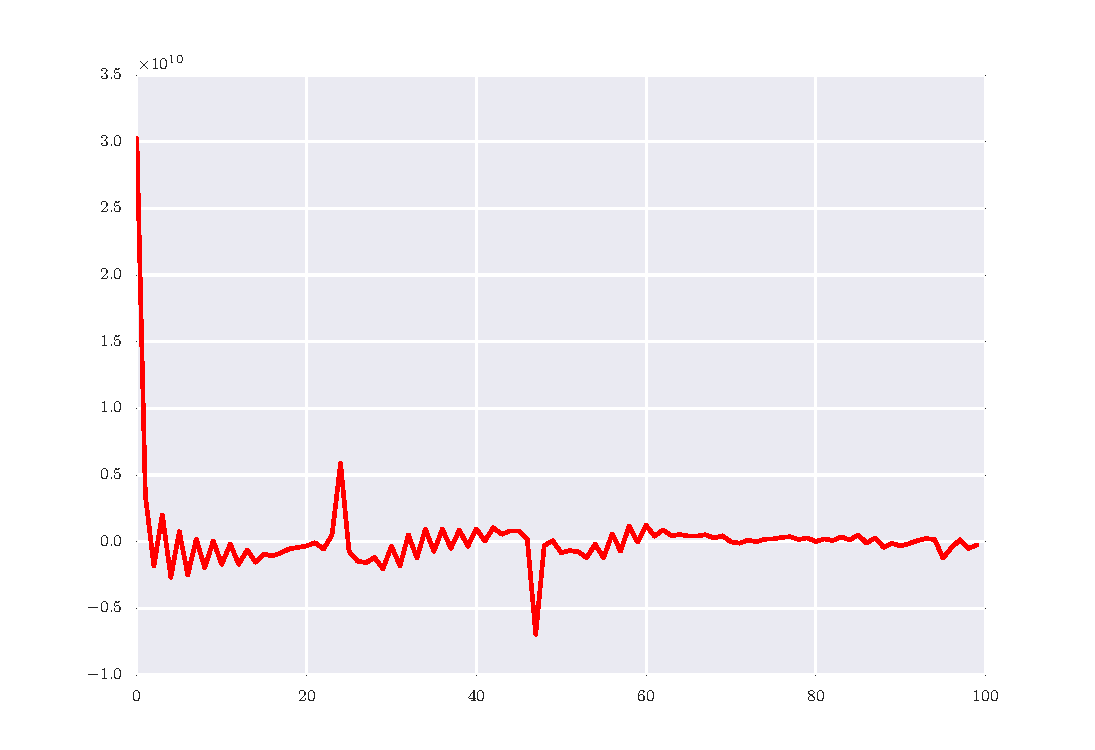
\includegraphics[width=0.5\textwidth]{../Figures/Behaviors/kedft.pdf}
\caption{Kinetic energy and discrete Fourier transformation of the same signal.}
\end{subfigure}
\caption{Observed behaviors of the soft robots used for the sparsity computation in novelty search.}
\label{fig:Behaviors}
\end{figure}
%The behaviors designed to describe the strategy and the efficiency of the evolved locomotion strategies. 
%They contain information that indirectly implies both the objectives of the evolution. 
%Trajectories, either in 2D or 3D, indirectly contain information about speed, displacement, and the deployed locomotion strategy. 

In order to compute the novelty measure~(see Equation~\eqref{sparsenessEquation}) for a trajectory behavior, we need to define the distance function $dist$. By definition, all trajectories start at the origin and trajectory points are sampled at the same constant rate. Trajectories are rotated so that the average over all trajectory points falls on the $x$--axis, thus resulting in a rotation--invariant measure. Hence, the difference in two behaviors $\mathcal{S}_i$ and $\mathcal{S}_j$ can be computed as the sum over the point absolute differences between the corresponding trajectories $\bm{t}_i$ and $\bm{t}_j$: 
\begin{align}
\mathcal{S}_i &= \bm{t}_i = t_{i,1}, t_{i,2}, \ldots, t_{i,N}\\
\mathcal{S}_j &= \bm{t}_j = t_{j,1}, t_{j,2}, \ldots, t_{j,N}\\
dist(\mathcal{S}_i, \mathcal{S}_j) &= \bm{t}_i - \bm{t}_j = \sum_{k=1}^{N} \left\lVert t_{i, k} - t_{j, k} \right\rVert
\end{align}
where $N$ is the number of sampled coordinate points. In the same way we can define the distance between other types of behaviors and subsequently compute the sparseness (see Equation~\eqref{sparsenessEquation}) a.k.a the novelty measure. For the discrete Fourier transformation of the one dimensional signals only the absolute difference in the first twenty coefficients is measured.

%Apart from trajectory type behaviors, pace, voxels touching the ground, kinetic energy, pressure, as well as, the discrete Fourier transformation of these signals were used to define other behavior types. The similarity or the difference of two of the same type behaviors can be determined by the equations provided while these measures of difference are used by the sparsity equation (see Eq.~\ref{sparsenessEquation}) to compute the sparseness of a given behavior in the behavior space. Individuals with novel observed behaviors (high sparseness value) are then stored in a list helping the evolution to avoid generating similar behaviors.


\subsection{Fitness--elitism in novelty search}
While novelty search promotes diversity by rewarding novel individuals, elitism ensures that the best genetic material is passed on from generation to generation. In particular, we introduce elitism in CPPN-NEAT by carrying--over the best individual of each species so that they can contribute with their beneficial genes later in the evolutionary process. We distinguish between fitness--elitism, where the ``best'' individuals are selected based on the fitness function and novelty--elitism, where the individuals with the highest sparseness are protected from modification. When combining fitness--elitism with novelty search, the fittest individual is carried over to the next generation and serves in the gene pool to possibly spawn novel yet fit individuals thus combining the best of both worlds, process similar to novelty--based multiobjectivization~\cite{mouret2011novelty}. Going forward, we deploy novelty search with and without fitness--elitism to study the effectiveness of this approach.

%Novelty search can include elitism in its selection process, and it does that by copying the most novel organisms of the current population of each species to the next while the same function can also be used to copy fit individuals within novelty search method. 
%The way these two elitism functions can be combined together depends on the population size and the problem, while probabilistic methods can also be applied. In the specific setting, both elitism function copy new individuals to the new generation with probability one. Moreover, evolution towards novelty does not get disturbed, at the same time fit individuals have the chance to be optimized further as long as they are the fittest within the species population. 

\begin{figure}[t!]
\vspace{0.2cm}
\centering
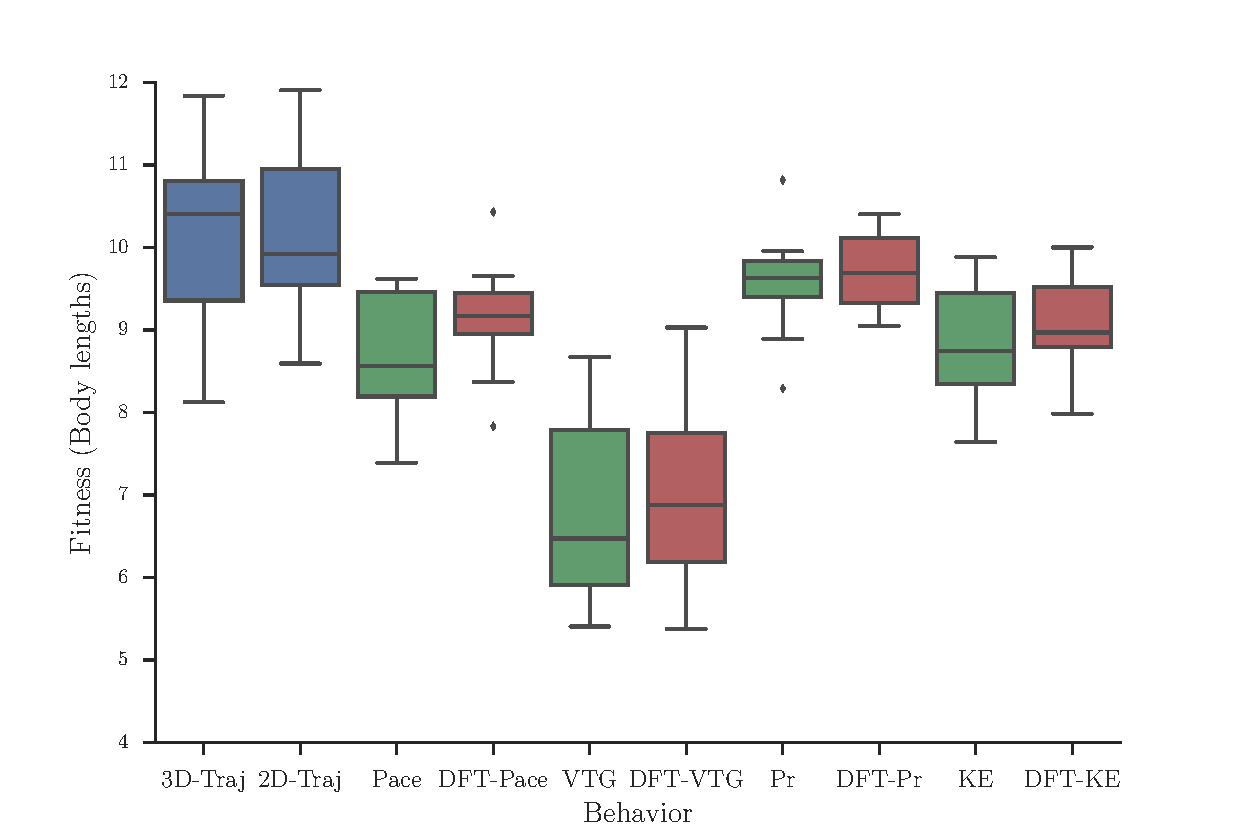
\includegraphics[width=0.5\textwidth]{../Figures/Results/BehaviorPerformanceNoveltyOnly.pdf}
\caption{Boxplots of the champion fitness under $10$ variant defined behaviors for novelty search. \textcolor{RoyalBlue}{Blue} are trajectory type behaviors (3D and 2D), \textcolor{ForestGreen}{green} are 1D signals (pace, voxels touching the ground (VTG), pressure (Pr), and kinetic energy (KE)). \textcolor{BrickRed}{Red} is the discrete Fourier transformation (DFT-<type>) of the 1D signals.}
\label{fig:BehaviorsPerformance}
\end{figure}

\subsection{Experimental setup}
Each experiment consists of $10$ runs with the following fixed settings. The population size is set to $30$ individuals and the maximum number of generations per run is set to $1000$. Due to the extremely computationally demanding simulations, not all experiments could be carried out using a VoxCad lattice of $10 \times 10 \times 10$, where applicable deviating dimensions are indicated. We use two externally activated materials with non-zero and opposite thermal expansion coefficients, colored \textcolor{Red}{Red} and \textcolor{Green}{Green}. The two additional materials represent non-actuated tissue, representing soft tissue (\textcolor{Cyan}{Cyan} voxels) with a five times smaller elastic modulus of their material than hard tissue (\textcolor{Blue}{Blue} voxels). % which have $50$ \texttt{MPa}.
For neuro-evoluation we use the HyperNEAT\footnote{HyperNEAT \texttt{v4.0 C++}  by J. Gauci code (url: \small{\url{ https://github.com/MisterTea/HyperNEAT})}} package; all parameter settings of CPPN-NEAT are the same as detailed in~\cite{cheney2013unshackling}. Details about the experimental setup, source code, and a wiki page on how to reproduce experiments can be found in  the project's repository\footnote{\small{\url{http://tinyurl.com/Soft-Robots-Novelty-Search}}}.


\section{Results}
Pure novelty search is compared with respect to the fitness measure (displacement of soft robots in body-lengths) to fitness--based search. Different behavior types are used to investigate the effects on performance of novelty search. In addition we explore the effect of fitness--elitism when combined with novelty search. Lastly, the performance of both methods, novelty and fitness--based search, are investigated for several levels of gravity. Evolved candidate solutions show how environmental conditions can have significant effect on the morphologies and the locomotion strategies of soft robots.


\begin{figure}[t!]
\centering
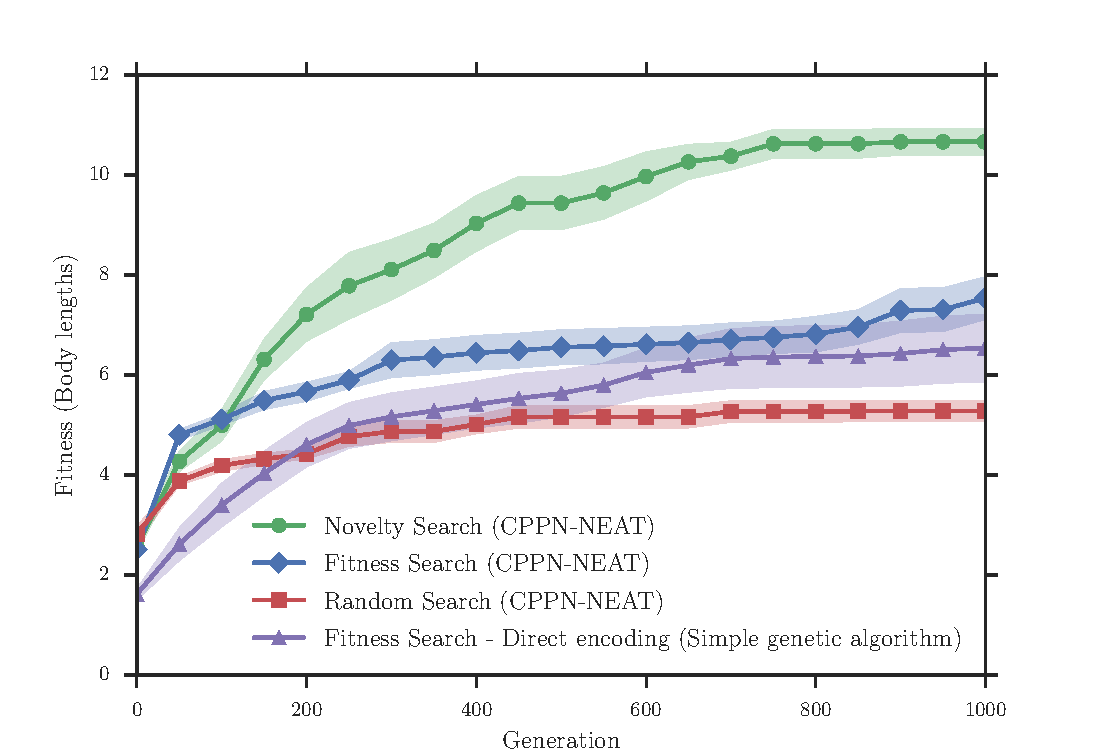
\includegraphics[width=0.5\textwidth]{../Figures/Results/FitNovRandomDirectSize5.pdf}
\caption{Comparison of simple genetic algorithm (direct encoding) against novelty-fitness-random search with generative encoding. Best fitness so far averaged over $10$ runs, deviation error is shown by the shaded part.}
\label{fig:FitNovRandomDirectSize5}
\end{figure}

\subsection{Behavior selection} 

Figure~\ref{fig:BehaviorsPerformance} illustrates the performance achieved by novelty search for the $10$ behavior types. In particular, what is shown is the fitness in body-lengths of the champion of the whole evolution for $10$ independent runs for a lattice size $7^3$. Both trajectory--type behaviors achieve the best performance with regards to the fitness measure, with a small difference in favor of 2D over 3D trajectories. The rest of the behavior metrics apart from VTG and DFT-VTG are close as far as the final performance of the evolution is concerned. One reason they fail to meet the trajectories' performance is the fact that although they keep track of cues that can describe the performance of the robot (e.g., displacement and speed), they cannot encode the direction of motion. Soft robots that have a circular trajectory can exhibit fast locomotion, in this case though, the measured displacement from their initial position remains low. Counting the number of voxels of a soft robot that touched the ground at every sampling step of the simulation does not hold any information as to how fast the robot is moving. A fast moving robot that is hopping can have a similar behavior to a hopping robot that stays in the same position. In contrast, the trajectory behavior of these robots would show a large difference.


\subsection{Performance comparison}
To compare the performance achieved by novelty search, its performance is set side by side with fitness--based search (normalized body-length displacement of the soft robot's center of mass from its initial position), random search, and finally a simple genetic algorithm\footnote{The GAlib C++ library \cite{wall1996galib} used for the implementation of this method. Source code used from~\cite{cheney2013unshackling}.} with direct encoded genomes. The same experiment held under two different simulation settings (i.e. for lattice size $5^3$ and $10^3$). Note, that the first three methods are referring to a generative encoding evolved by CPPN-NEAT and using selection with respect to novelty, fitness, and random selection. The last method uses a direct encoded genome driven by fitness within a simple genetic algorithm. Two dimensional trajectories are used by novelty search in order to describe the novelty in the behavior space through the sparseness measure.

\begin{figure}[t!]
\centering
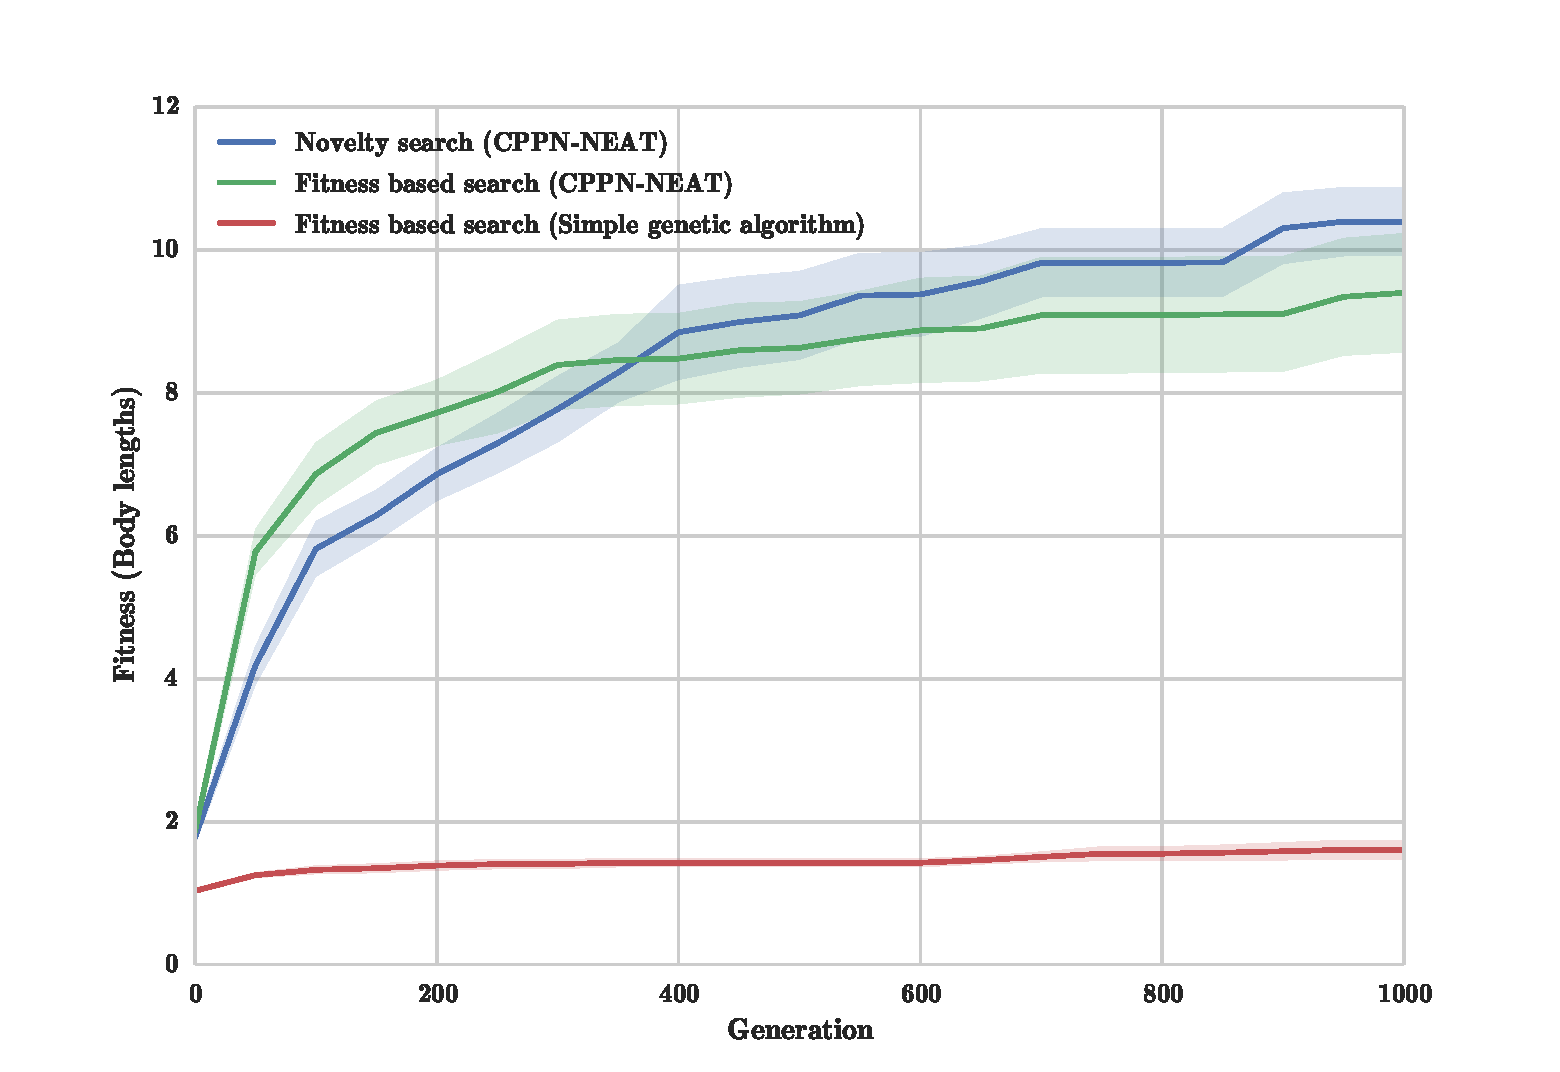
\includegraphics[width=0.5\textwidth]{../Figures/Results/FitvsNovVsDirSize10.pdf}
\caption{Simple genetic algorithm against novelty-fitness-random search with generative encoding. Best fitness so far averaged over $10$ runs.}
\label{fig:FitvsNovVsDirSize10}
\end{figure} 

Figure~\ref{fig:FitNovRandomDirectSize5} presents the results for the small lattice (i.e. $5^3$). The average best displacement so far is presented alongside the deviation error. Note, the difference between novelty search and the other methods. Using the two dimensional trajectories of the soft robots, novelty search visits optimal solutions that none other method reaches. Local optima can prevent fitness--based search to achieve the performance of novelty search. Encoding limitations in direct encoding cannot lead to optimal solutions for this settings. In the case of random search, having neither the information about their fitness, nor the driving force of novelty search that seeks for novel behaviors, it fails to evolve any successful locomotion strategy. The only reason random search in CPPN-NEAT achieves a displacement of $\sim 5$ body-lengths, is the powerful generative encoding. The simple genetic algorithm approach performs better than using random selection with an indirect encoding. Structural regularity and symmetry does not show all of its advantages in this small lattice setting.

For larger lattices, it is expected that generative encoding will prove its merits over the direct encoding scheme~\cite{cheney2013unshackling,stanley2007compositional}. More complicated morphologies can be produced (morphology space for $10^3$ lattice resolution: $9.3 \times 10^{698}$). Furthermore, the space of behaviors, for instance two dimensional trajectories, becomes larger since more complex soft robots can achieve higher displacement and more advanced strategies for locomotion. These higher resolution morphologies can achieve life--like locomotion. Figure~\ref{fig:FitvsNovVsDirSize10} illustrates the performance (i.e. best displacement so far) of the four different methods in these higher resolution settings. Results reassure that novelty search achieves higher fitness ($> 1$ body-length) on average against fitness--based search. Nevertheless, the effect is not as strong as in the previous experiment. Both methods succeed to evolve the soft robot structure with the highest fitness found in all experiments ($\sim 14$ body-lengths). Novelty search behaves more constant in evolving individuals with high fitness in all runs, on the other hand most of individual runs of fitness--based search are being trapped in low fitness local optima, trying to optimize specific individuals without trying to explore deeply the fitness landscape like novelty search successfully does. The high difference between random evolution and novelty search proves that seeking novel behaviors in novelty search cannot be considered as a random search. The superiority of generative encoding (i.e. CPPN) over direct encoding can be clearly observed. Regularity in shape morphologies provides advantages that result in more efficient motion.

\begin{figure}[t!]
\centering
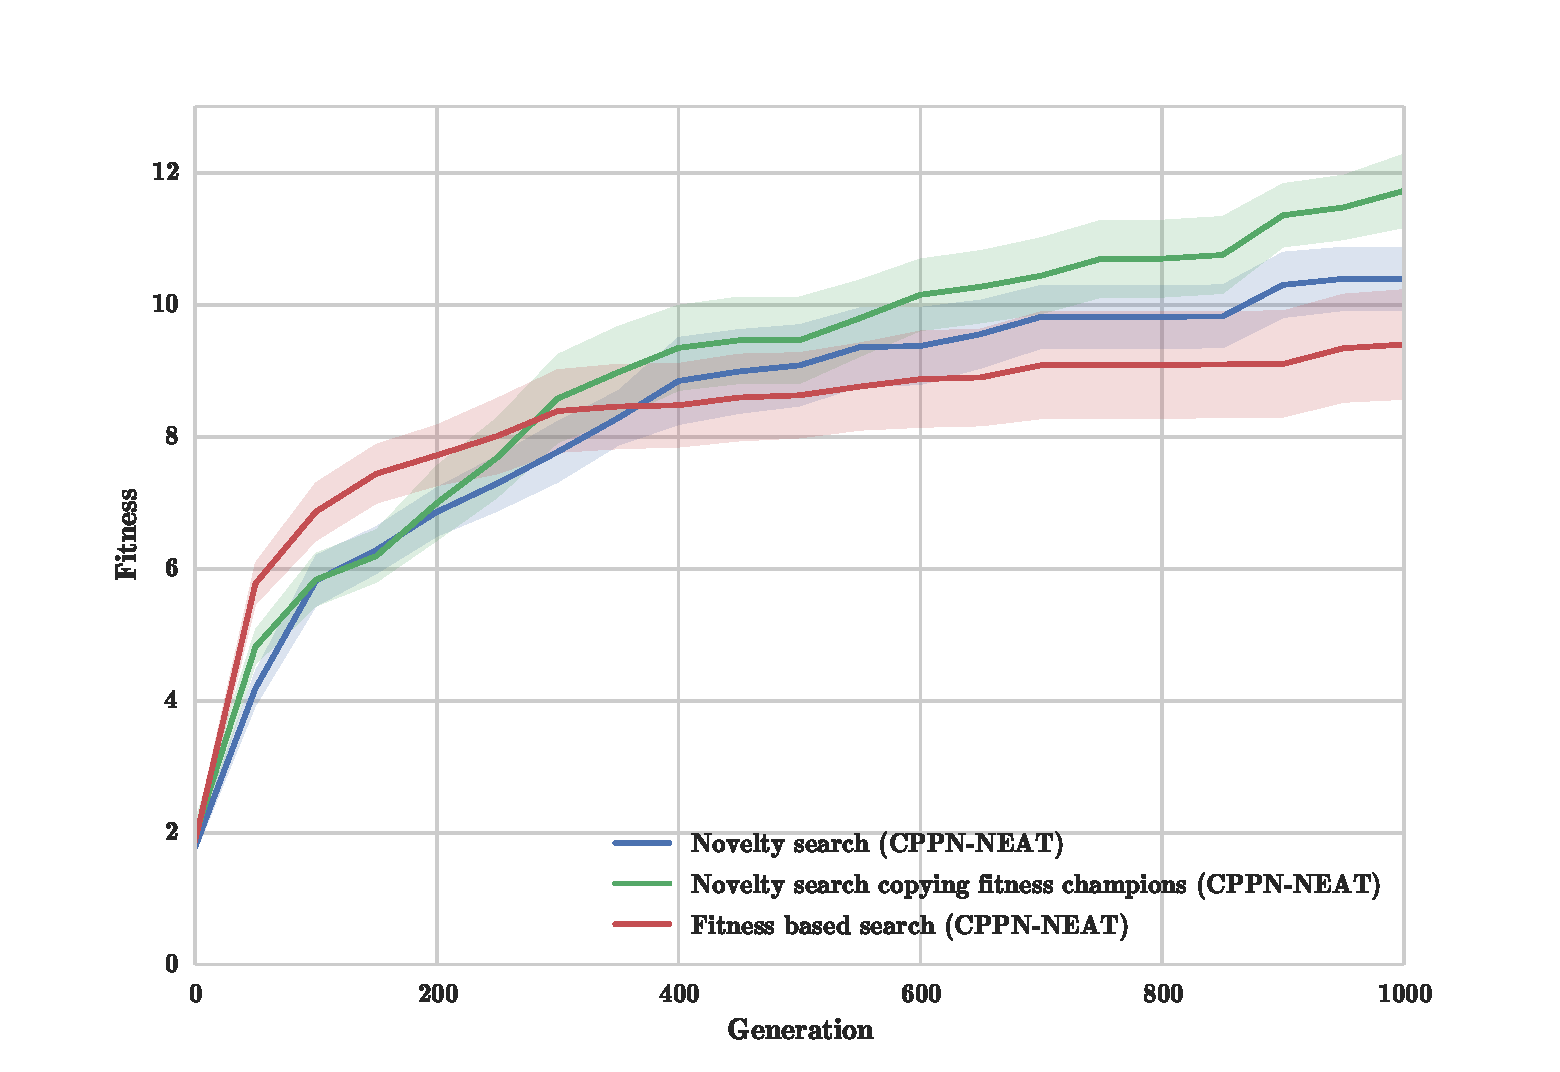
\includegraphics[width=0.5\textwidth]{../Figures/Results/CopyFitChampions10.pdf}
\caption{Best fitness so far, novelty search with and without copying \emph{fit} champions (fitness--elitism), and fitness search, averaged over $10$ runs.}
\label{fig:CopyFitChampions10}
\end{figure}


\subsection{Fitness--elitism in novelty search}
The reason that novelty search is considered such a revolutionary search method is because it finds solutions for deceptive problems, where the fitness landscape is not a straightforward function. At each generation of novelty search, novel behaviors that are also fit with regards to the objective of the problem are discovered. Mutations of these solutions will yield in behaving similarly to their ancestors, resulting in similar behaviors. Thus, the novelty value of these individuals will be declined as similar behaviors will contribute in a denser area in the behavior space. Eventually, these solutions will stop being selected, and evolution will not have the chance of carrying their genes along. Mutations and other genetic operations can optimize these fit individuals more. These individuals (with high fitness values) can be seen as \emph{stepping~stones}~\cite{lehman2011abandoning} towards more optimized versions of themselves. Being blind to the objective function, novelty search will eventually stop producing new individuals out of them, which will lead to promising individuals being unable to survive through the evolution process. Figure~\ref{fig:CopyFitChampions10} illustrates the gain in performance when fitness--elitism is used in novelty search method compared with the pure novelty and fitness--based search methods.


\section{Evolving Soft Robots for Space Exploration} 

\begin{figure}[t!]
\centering
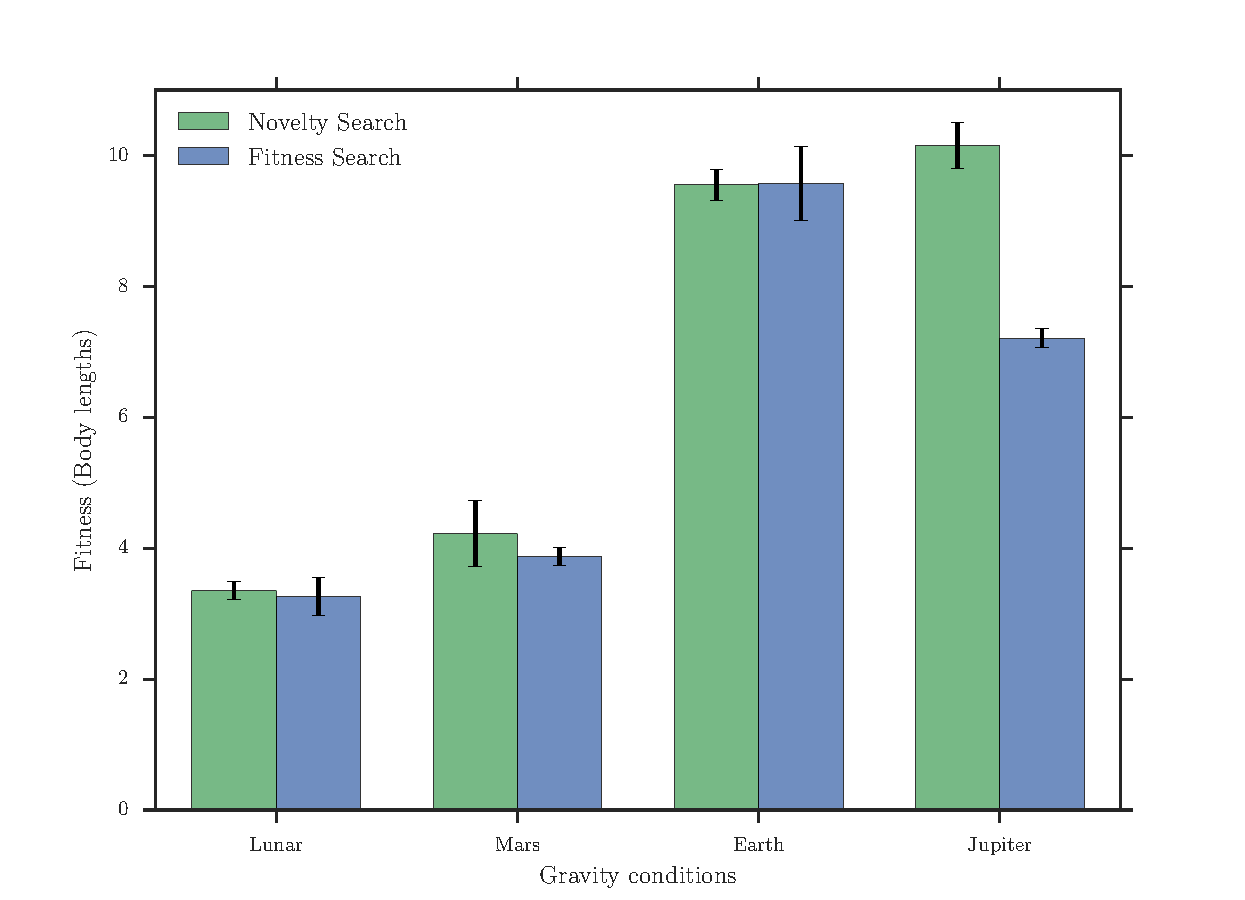
\includegraphics[width=0.5\textwidth]{../Figures/Results/GravityExperiment.pdf}
\caption{Novelty search performs better or equally good than fitness--based search in all gravity conditions tested.}
\label{fig:gravityConditions}
\end{figure}

Gravity conditions heavily affect the evolution of soft robots in our set-up. The interaction between the robot body and the environment biases the selection towards chromosomes that are able to produce robot bodies that efficiently interact with the terrain at the considered gravity strength. We experiment with both methods discussed, novelty and fitness--based search. For the novelty search method we select the two dimensional trajectories of the soft bodies as the behavior metric defining the novelty of each individual. Figure~\ref{fig:gravityConditions} presents the performance of novelty and fitness--based search for four different gravity levels using a lattice size $7^3$.

\subsubsection*{Soft robots on Lunar's Gravity}

Locomotion strategies evolved under Lunar gravity showed that only hopping gaits can produce effective locomotion. Low gravity makes it difficult for the soft body structures to grip on the ground surface and evolve different strategies than hopping. The morphology of each hopper differs. A C-shaped hopper soft robot (see Fig.~\ref{fig:gravityRobots1.6-4}) evolved in these settings.

\subsubsection*{Soft robots on Mars' Gravity}

The locomotion effectiveness on Mars is higher when compared to Lunar, higher gravity acceleration makes it possible for the virtual soft robots to evolve other kind of gaits using legged bodies (see Fig.~\ref{fig:gravityRobots3.7-2}). Note that the C-shaped hopper soft robot mostly uses passive materials apart from its upper body where all the active material are located. Its upper part alone generates enough motion to hop efficiently. What is observed in the morphologies evolved at lower gravity levels is that the use of a lower number of active voxels can still produce decent locomotion.

\subsubsection*{Soft robots on Earth's Gravity}

On higher gravity levels familiar locomotion strategies emerge. In Figure~\ref{fig:hildebrand} we show the Hildebrand diagram for two of the creatures evolved under Earth gravity, where we note characteristics remarkably similar to biped and quadruped locomotion used by animals on Earth. Interesting animal-like gaits are visualized in Fig.~\ref{fig:gravityRobots9.8-2}. These results suggest an encouraging connection between our set-up and the locomotion strategies of living organisms evolved on Earth for thousands of years. Tumbleweed-like locomotion (see Fig.~\ref{fig:gravityRobots9.8-3}) has also emerged at this gravity level under novelty search, producing rolling soft robots that can locomote efficiently. 
%This adds significance to the novelty search method since fitness--based search did not produce this kind of locomotion strategy. 
Tumbleweed is also a concept of low-cost exploration that has inspired robot designers for Mars' missions in the past~\cite{antol2003low} and has been already deployed in Antarctica for testing purposes by NASA.

\begin{figure}[t!]
\vspace{.5cm}
\centering
\begin{subfigure}[b]{0.5\textwidth}
\centering
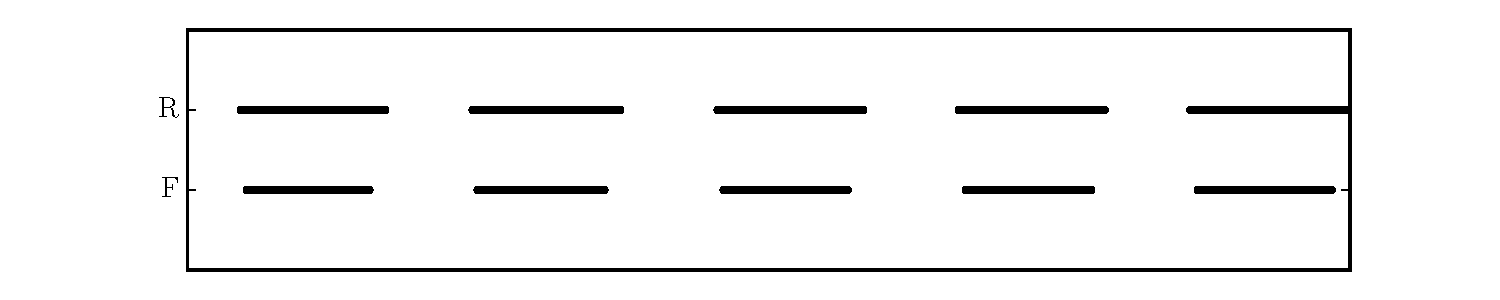
\includegraphics[width=1.0\textwidth]{../Figures/Results/hildebrand1.pdf}
\caption{Two-legged soft robot.}
\vspace{.63cm}
\end{subfigure}
\begin{subfigure}[b]{0.5\textwidth}
\centering
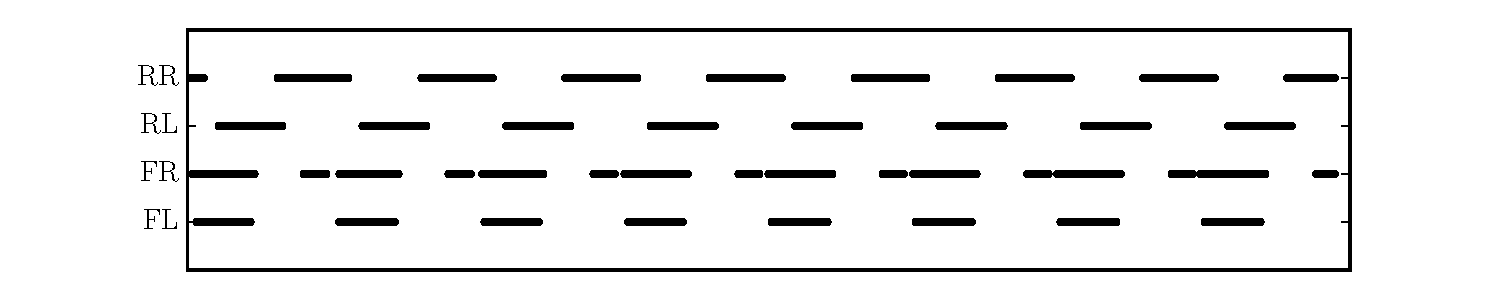
\includegraphics[width=1.0\textwidth]{../Figures/Results/hildebrand2.pdf}
\caption{Four-legged soft robot.}
\vspace{.62cm}
\end{subfigure}
\caption{Hildebrand diagrams of two evolved soft robots for Earth's gravity acceleration. Timing of impacts between its legs and the ground.}
\label{fig:hildebrand}
\end{figure}


\subsubsection*{Soft robots on Jupiter's Gravity}

Moving on to higher gravity levels, i.e. on Jupiter, heavier structures can use galloping as a strategy for their locomotion. Galloping is again considered to be an effective way of moving in such a high gravity, whereas thicker legs are evolved to withstand the high gravitational force. Push-pull worm-like locomotion can also produce decent velocities for soft robots. Finally, hoppers have also evolved in this setting (performing short hops), while using more actuated materials (see Fig.~\ref{fig:gravityRobots27.6-3}).

\begin{figure*}[t!]
\centering
\begin{subfigure}[b]{1.0\textwidth}
\centering
\foreach \i in {2,3,4,5,6,8,9}{ 
\includegraphics[width=0.14\textwidth]{../Figures/Robots/moon-nov-g1-2-\i.jpg}\hspace{-0.16cm}
}
\caption{Lunar's gravity: C-shaped hopper (Novelty search)}
\label{fig:gravityRobots1.6-4}
\end{subfigure}
\begin{subfigure}[b]{1.0\textwidth}
\centering
\foreach \i in {1,2,3,4,5,7,8}{ 
\includegraphics[width=0.14\textwidth]{../Figures/Robots/mars-nov-g3-1-\i.jpg}\hspace{-0.16cm}
}
\caption{Mars' gravity: 2-legged C-shaped hopper (Novelty search)}
\label{fig:gravityRobots3.7-2}
\end{subfigure}
\begin{subfigure}[b]{1.0\textwidth}
\centering
\foreach \i in {1,2,3,4,5,6,7,8,9,10}{ 
\includegraphics[width=0.097\textwidth]{../Figures/Robots/grass-fit-g9-2-\i.jpg}\hspace{-0.16cm}
}
\caption{Earth's gravity: \emph{Top view}, 4-legged animal like locomotion (Fitness search)}
\label{fig:gravityRobots9.8-2}
\end{subfigure}
\begin{subfigure}[b]{1.0\textwidth}
\centering
\foreach \i in {1,2,3,4,5,7,8}{ 
\includegraphics[width=0.14\textwidth]{../Figures/Robots/grass-nov-g9-1-\i.jpg}\hspace{-0.16cm}
}
\caption{Earth's gravity: Tumbleweed-like locomotion (Novelty search)}
\label{fig:gravityRobots9.8-3}
\end{subfigure}
\begin{subfigure}[b]{1.0\textwidth}
\centering
\foreach \i in {1,2,3,7,8,9,10}{ 
\includegraphics[width=0.14\textwidth]{../Figures/Robots/gas-nov-g2-1-\i.jpg}\hspace{-0.16cm}
}
\caption{Jupiter's gravity (Assuming a stable surface): C-shaped hopper (Novelty search)}
\label{fig:gravityRobots27.6-3}
\end{subfigure}
\caption{Locomotion strategies evolved in variant gravity conditions.}
\label{fig:gravityRobots1.6}
\end{figure*}

\section{Discussion and Outlook}
In all our experiments, both novelty search and fitness search evolved soft bodies able to efficiently move in the considered environment. However, the performance with regard to the fitness defined (i.e. displacement of the body in body-lengths) was equal or higher for novelty search in all experiments. One would expect novelty to deliver more diversity, at the cost of a lower fitness function; novelty does not know about fitness and a method well targeted to improve fitness is likely to deliver better results. This was not the case and we found that the creatures evolved with novelty are also able to move faster than the ones that were evolved to move fast. Previous work~\cite{lehman2011evolving} in a try to evolve walking three dimensional virtual creatures used the evolved morphology of the creatures to describe their behavior. Although, comparing the morphology of the evolved soft robots is similar to comparing the chromosome (CPPN) of each individual. Behaviors that describe the morphology of the evolved robots have failed~\cite{lehman2011evolving}, since search is then forcing new types of morphologies without caring about the actual target of the evolution, which was the efficient locomotion. Therefore, only the comparison of the observed behavior in the phenotype level can lead the evolution towards more complex behaviors. 

Some interesting general observations can be made. To start with, low gravity levels seem not to allow for a great variety of gaits. Hopping seems to be the predominant strategy followed by most evolved creatures. Higher gravity levels, instead, allow for more complicated behaviors to emerge and legged locomotion starts to became favorable. At Earth gravity levels, gaits remarkably similar to animal-like motion appear, increasing our confidence in the simulation set-up. Second, the greater variety of creatures evolved using novelty search, allow for rolling tumbleweed-like~\cite{antol2003low} robots, quadruped and biped robots, hoppers as well as odd creatures to emerge. 

Beyond its purely inspirational value, we believe that this methodology, if improved and refined, can be of direct use for the design of soft robotic rovers. Extreme temperature fluctuations, for example on asteroids or comets, could trigger passive actuated materials to perform a designed movement. Although the VoxCad simulator could not be used to simulate the extreme environment of asteroids or comets, it is an interesting idea for further research. The rotation of the celestial body (e.g., with a period as short as a few hours) would then create a cyclic temperature profile having an extreme excursion and thus actuating the soft robot locomotion. This would result, if the soft robot was evolved in such an extreme environment, into a slow crawl of the robot leading to an extremely useful exploratory behavior that could deliver incredible scientific data. %We just have to imagine what would it be like if Philae~\cite{glassmeier2007rosetta}, the robotic-probe landed on comet 67P was just now be slowly crawling around 67P.
\newpage
\section{Conclusions}
We introduced the use of a diversity seeking method, novelty search, in evolutionary soft robotics. 
%Novelty search was found to outperform traditional fitness based search in evolving soft robotic morphologies with respect to the fitness criteria as well as with respect to the diversity criteria. 
%Previous work in evolving virtual creatures by novelty search~\cite{lehman2011evolving} used the resulted morphology of the robots created to determine the novelty of an individual. 
%The resulted performance for pure novelty search method was worse than the fitness--based. 
We found that well defined behavior metrics can lead novelty search to outperform traditional fitness--based search. Novelty search not only improved the performance and the diversity in the fitness space, but also contributed to a larger variety of morphologies. Finally, both techniques were used to evolve soft robots in four different gravity levels, showing interesting results and the possibility of influencing future robotic designs for planetary exploration.

\bibliographystyle{unsrt}
\balance
\bibliography{bibliography}

\end{document}
